\subsection{Electrophysiology of Speech Perception}

The human auditory system is sensitive to within-category distinctions 
in speech sounds, and such pre-categorical perceptual distinctions may 
be lost in transcription tasks, where listeners must filter their 
percepts through the limited number of categorical representations 
available in their native language orthography. 
EEG distribution coding is a proposed new method that interprets the
electrical evoked potentials of untrained listeners
(measured by an electro-encephalograph or EEG) as a posterior
probability distribution over the phone set of the utterance language
(Fig.~\ref{fig:eeg_paradigm}).  Transcribers, in this scenario, listen
to speech in both their native language and an unfamiliar non-native
target language, while their EEG responses are
recorded.  From their responses to English speech, an English-language
EEG phone recognizer is trained, using methods based
on~\cite{Liberto15}.  Misperception probabilities $\rho(\psi|\phi)$
are then estimated: for each non-native phone $\phi$, the
classifier outputs are interpreted as an estimate of $\rho(\psi|\phi)$
for all $\phi\in\mathbb{\Phi}$, the native phone inventory.

\begin{figure}
  \centerline{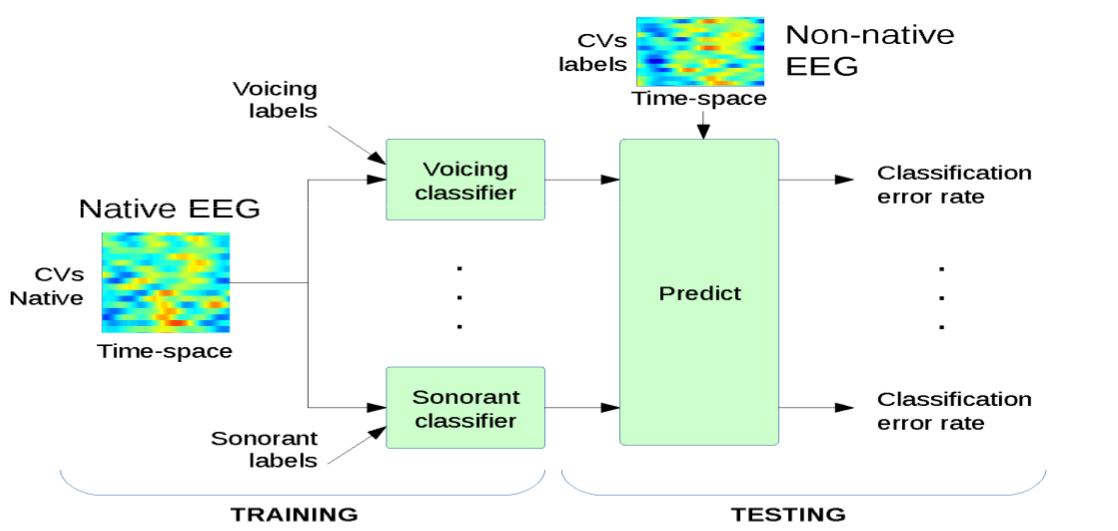
\includegraphics[width=4in]{../figs/diliberto_paradigm.png}}
  \caption{EEG responses are recorded while listeners hear speech in
    their native language and an unfamiliar non-native language.  For 
    each listener, a bank of distinctive feature classifiers are trained. 
    Those classifiers are then applied to the EEG responses to non-native
    speech, estimating a listener-language transcription of the
    non-native speech.}
  \label{fig:eeg_paradigm}
\end{figure}
